\begin{figure}[tb]
  \centering
  \begin{subfigure}{0.31\linewidth}
 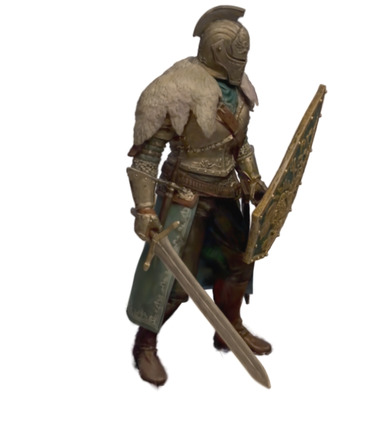
\includegraphics[width=\linewidth]{images/artifacts/static.jpg}
 \caption{\tiny Original pose}
  \end{subfigure}
  \hfill
  \begin{subfigure}{0.31\linewidth}
  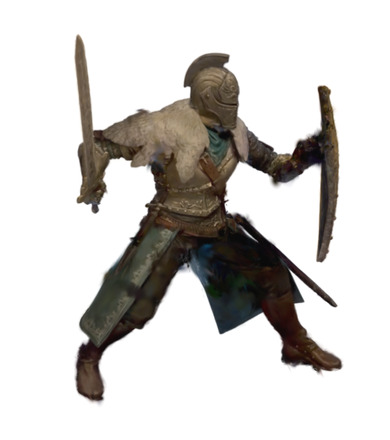
\includegraphics[width=\linewidth]{images/artifacts/no_artifact.jpg}
  \caption{\tiny Adaptive thickness (ours)}
  \end{subfigure}
  \hfill
  \begin{subfigure}{0.31\linewidth}
  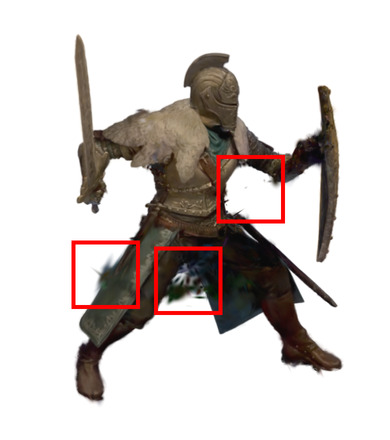
\includegraphics[width=\linewidth]{images/artifacts/with_artifact_0.jpg}
  \caption{\tiny Constant thickness (baseline)}
  \end{subfigure}
  %
  \caption{
  \textbf{Comparison with a constant thickness.} Our strategy to compute an adaptive thickness for Frosting is essential to maintain optimal performance while avoiding artifacts when editing the scene. As shown in the right image, using a constant thickness may produce artifacts when animating a character: When using a constant, large thickness in this scene, Gaussians located near the right knee of the knight participate in reconstructing the right hand, which produces artifacts when moving the hand.
  }
  \label{fig:artifacts}
\end{figure}